\section{Nondeterministic automata}

A right-linear grammar may contain two alternative rules starting with the same character. In this case, converting the rules to machine transitions, two arrows with 
identical label would exit from the same state $A$ and enter two distinct states $B$ and $C$. This means that in state $A$, reading the character, the machine can 
choose which one of the next states to enter: its behavior is not deterministic. A machine move that does not read an input character is termed spontaneous or an epsilon 
move. Spontaneous moves too cause the machine to be nondeterministic. 

\subsection*{Motivation of non-determinism}
The main advantages of this are: 
\begin{itemize}
    \item Concision: defining a language with a nondeterministic machine often results in a more read-able and compact definition. 
    \item Left right interchange and language reflection: it is useful when a deterministic machine is used to recognize the reflection. 
    \item Converting regular expressions to automaton. 
\end{itemize}

\subsection*{Nondeterministic recognizers}
\begin{definition}
    A \emph{non-deterministic finite automaton} $N$, without spontaneous moves, is defined by: 
    \begin{itemize}
        \item The state set $Q$. 
        \item The terminal alphabet $\Sigma$. 
        \item Two subsets of $Q$: the set $I$ of the initial states and the set $F$ of final states.
        \item The transition relation $\delta$, a subset of the Cartesian product $Q\times\Sigma\times Q$.     
    \end{itemize}
\end{definition} 
As before, a computation is a series of transitions such that the origin of each one coincides with the destination of the preceding one. The computation
origin is $q_0$, the termination is $q_n$, and the length is the number $n$ of transitions or moves. A computation of length 1 is just a transition.
A string $x$ is recognized or accepted by the automaton, if it is the label of a computation originating in some initial state, terminating in some final state, 
and having label $x$. The language $L(N)$ recognized by automaton $N$ is the set of accepted strings. The moves of a nondeterministic automaton can still be 
considered as a finite function, but one computing sets of values. For a machine $N=(Q,\Sigma,\delta,I,F)$, devoid of spontaneous moves, the functionality of the 
state-transition function $\delta$ is the following: 
\[\delta:Q\times\left(\Sigma\cup\{\varepsilon\}\right)\rightarrow \mathcal{P}(Q)\]
where symbol $\mathcal{P}(Q)$ indicates the power set of set $Q$. 

\subsection*{Automata with spontaneous moves}
Another kind of nondeterministic behavior occurs when an automaton changes state without reading a character, thus performing a spontaneous move. In this case 
the number of steps of the computation can exceed the length of the input string, because of the presence of $\varepsilon$-arcs. As a consequence, the recognition 
algorithm no longer works in real time. Yet time complexity remains linear, because it is possible to assume that there are no cycles of spontaneous moves in any 
computation. The family of languages recognized by such nondeterministic automata is also called finite-state.

The official definition of nondeterministic machine allows two or more initial states, but it is easy to construct an equivalent machine with only one: add to the
machine anewstateq0, which will be the only initial state, and the $\varepsilon$-arcs going from it to the former initial states of the automaton.

\subsection*{Correspondence between automata and grammars}
Consider a right-linear grammar $G=(V,\Sigma,P,S)$ and a nondeterministic automaton $N=(Q,\Sigma,\delta,q_0,F)$, which we may assume from the preceding discussion to 
have a single initial state. First assume the grammar rules are strictly unilinear. The states $Q$ of the automaton match the non-terminals $V$ of the grammar. The 
initial state corresponds to the axiom. Notice that the pair of alternatives $p\rightarrow aq|ar$ correspond to two nondeterministic moves. A copy rule matches a 
spontaneous move. A final state  matches a non-terminal having an empty rule.
\begin{figure}[H]
    \centering
    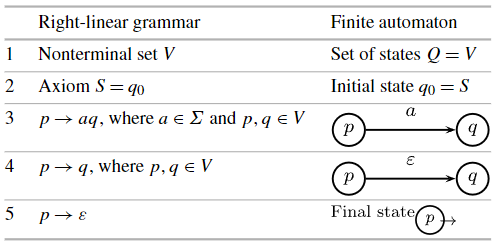
\includegraphics[width=0.75\linewidth]{images/correspondence.png}
    \caption{Correspondence between automaton and grammar}
\end{figure}

\subsection*{Ambiguity of automata}
\begin{definition}
    An automaton is \emph{ambiguous} if it accepts a string with two different computations.
\end{definition}
Clearly it follows from the definition that a deterministic automaton is never ambiguous. We also have that an automaton is ambiguous if, and only if, the right-linear 
equivalent grammar is ambiguous. 

REG families can be defined also using left-linear grammars. By interchanging left with right, it is simple to discover the mapping between such grammars and automata.